\chapter{独立序列型数据属性隐私推断模型}
\label{chap:inference-attack-on-norelated-sequenced-data}

\textit{ }

\textit{基因序列数据、连续轨迹位置数据等呈现序列化,此类数据在很多共享应用场景(如疾病诊断、车联网导航)中需要非匿名化,需要对其敏感的属性隐私(特定基因座的基因型,特定行车位置)进行保护。保护这些隐私,需要更加深刻的理解隐私泄露的原因。本章针对基因序列数据的基因座值属性隐私,通过对单条敏感数据记录属性值存在的相互关联关系进行分析,构建目标属性值推断的敌手模型,并以此为基础利用抽样、隐Markov推断、卷积神经网络构建概率推断算法,针对不存在亲属关系的群体型基因序列数据共享场景,分析属性隐私泄露情况,通过量化隐私泄露量和敌手获取隐私量等信息,提高对序列型数据属性隐私的认识和理解。
}

\section{概述}\label{sec:intro}

随着测序技术的进步,人们能够更轻松、更便宜地对其DNA进行测序,人类基因组数据已变得越来越可负担和可用。例如,在1000 Genomes项目~\cite{gpc2015global}中,数千名匿名参与者将其DNA数据捐献给了生物医学和精准医学研究。美国、英国、加拿大、法国和中国政府也出于医学和其他原因启动了基因组数据采集项目。此外,越来越多的人,因为娱乐、找与自己相似的病人、或找自己的亲属等原因,通过23andMe.com、PatientsLikeMe.com和Ancestry.com等网站在线分享他们的基因组数据。同时,通过基因组数据可以唯一确定识别一个人,也可以通过基因组数据识别特定的表现型和疾病。然而,基因组数据可用性的提高带来了更加突出的安全和隐私挑战。一旦这些数据被披露或滥用,一个人就可能会面临就业、保险、教育等多方面的歧视风险~\cite{eeoc2008genetic}。

实际上,许多研究结果和实际案例已经引起人们对基因组数据的机密性和隐私性的担忧。在某些情况下,以匿名方式收集的基因组数据仍可能以各种方式泄露个人的敏感信息。例如,Sweeney等~\cite{sweeney2013identifying}通过将个人基因组计划中不公开的姓名和联系信息链接起来,重新识别个体;Gymrek等~\cite{gymrek2013identifying}通过分析~$~Y~$~染色体上的短串联重复序列,重新识别个体。全基因组关联研究(Genome-Wide Association Study,GWAS)的结果可用于识别个体~\cite{cai2015deterministic}。某些疾病的易感性~\cite{shringarpure2015privacy}和基因表现型外观特征~\cite{walsh2011irisplex}也可以从基因组数据中推断出来。个人基因组数据的泄露不仅会对其个人隐私造成威胁,而且还会以家族身份~\cite{rohlfs2012familial}或有关亲属基因型信息的形式对其亲属的隐私造成威胁~\cite{humbert2013addressing}。最近,已经证实遗传学家可以从基因组数据中恢复特定个体的面孔~\cite{hess2017controversial},共享的基因组数据也有可能被恶意机构滥用~\cite{scutti2018what}。

实际情况可能会更糟,为了保护个人自身的基因组隐私,通常其可以选择删除或隐藏其基因序列的某些部分~\cite{shi2017overview},只向第三方(如医院或基因组研究机构)共享部分基因组数据。许多没有亲戚关系的人可以通过这种方式共享他们的基因组数据,这种方式看起来似乎是安全的,但其实不然。在本章中,我们将揭示敌手可以利用该个体的共享部分基因组数据和其他公开可用的基因组数据,稳健地重构个体的基因组数据。

在本章中,我们提出两种用于重构单个基因型序列的推断攻击方法:一种基于改进的离散隐Markov模型(Improved Hidden Markov Model, iHMM),另一种基于回归卷积神经网络(Convolutional Neural Network, RCNN)模型。这些推断攻击模型既考虑了观察到的被攻击者基因组数据,也考虑了公开可用的基因组数据。基于第\ref{chap:entropy-metric-model}章所提出的隐私度量模型提出了基因序列属性隐私度量指标,以量化被攻击者的基因组隐私以及有关不正确性、不确定性和隐私损失的攻击的严重程度。与Samani等~\cite{samani2015quantifying}先前的工作相比,本章的贡献如下:
\begin{itemize}
	\item 提出一个针对基因组隐私推断攻击的统一敌手模型,目的是从被攻击者部分观察到的基因组数据中重建不相关个体的基因型序列。
	\item 提出一种针对不相关个体的基因组隐私推断攻击策略,该策略利用IMPUTE2~\cite{howie2009flexible}中单核苷酸多态性(SNP序列)和抽样重组模型方法进行关联分析。
	\item 针对不相关个体的基因组隐私,提出一种基于RCNN模型的属性隐私分析推断攻击方法,并研究在基因组隐私攻击背景下机器学习(例如RCNN)的大规模隐私分析攻击功能。
	\item 从信息量的角度量化隐私推断攻击强度、量化基因隐私量,其代表了攻击者对隐私信息不确定程度的降低和被攻击者基因隐私损失量的增加。
	\item 提出的方法对基因序列属性隐私推断结果错误率更低,敌手推断获得的隐私不确定性更低,被攻击者的隐私信息损失更多。
\end{itemize}

\section{相关工作}\label{sec:relat}
\subsection{基因序列隐私推断攻击}

推断攻击利用可用数据通过数据分析来推断潜在的私人信息~\cite{en2018inference},是一种非常有效的隐私和安全攻击策略。推断攻击在位置跟踪~\cite{narain2016inferring}、社交网络上的属性隐私~\cite{gong2016you}、机器学习中的成员和属性隐私~\cite{shokri2017membership,ganju2018property}、高级密码学的脆弱性(例如,加密数据库和可搜索加密)~\cite{pouliot2016shadow} 和基因组隐私(例如,成员基因组隐私~\cite{wang2009learning}、基因型隐私~\cite{samani2015quantifying,he2017addressing}和亲属隐私~\cite{humbert2013addressing})。如文献~\cite{ayday2017inference}所述,推断攻击对社交网络,基因组共享,GWAS研究和临床医学等领域的基因组数据构成了巨大的隐私威胁。

本章中,我们重点研究基于被攻击者的共享SNP数据(其中隐藏了敏感的SNP数据)和公开可用的基因组数据,如何分析推断被攻击者的基因序列属性隐私。

\subsection{基因组数据隐私泄露}

尽管诸多文献关注统计基因组隐私的泄露问题,但其中大多数都与去匿名化的个体识别隐私有关,并依赖于成对连锁不平衡(Linkage Disequilibrium,LD)。Homer等~\cite{homer2008resolving}对GWAS统计数据进行的遗传隐私研究表明,可以从参与人的基因型推断出GWAS其疾病状态,人们开始考虑不再为GWAS研究和医学测试捐赠基因组数据。随后,去身份识别被认为不足以保护遗传隐私和机密性,许多公开数据库,例如美国国立卫生研究院(NIH)的基因型和表现型数据库(dbGaP)~\cite{mailman2007ncbi,nhgri2015privacy},访问规则已更改为根据其基因组数据需求进行控制性访问。Wang等~\cite{wang2009learning}的研究结果表明,GWAS结果可以推断个人身份和疾病。尽管公开GWAS目录中的数据经过差分隐私保护的,但其仍包含GWAS参与者的个人特征和身份,可以通过基于背景信息的挖掘来攻击个人的这些隐私~\cite{wang2016infringement}。通过使用公开的性状位点和基因表现型数据集,也可以通过将表现型与基因型联系起来分析获取个体的遗传隐私~\cite{harmanci2016quantification}。

本章的研究重点是基因型的隐私性,而不是基于基因组数据的身份隐私~\cite{wang2009learning,wang2016infringement}或疾病状态隐私~\cite{homer2008resolving,wang2009learning}。尽管我们的工作也是针对公开可用的基因组数据,但并不需要像文献~\cite{wang2009learning,wang2016infringement,harmanci2016quantification}中那样需要性状位点和表型现型数据。我们仅需通过基因共享网站(例如,PatientsLikeMe.com和23andMe.com)捐赠的可观测SNP序列数据以及来自基因研究项目(例如,HapMap项目和1000基因组计划)的公开基因组数据,即可建立隐私分析攻击模型获取基因型隐私信息。

在文献~\cite{schadt2012bayesian}中,作者提出了一种利用基因表达数据推断特定位点个体基因型的贝叶斯方法。Humbert等~\cite{humbert2013addressing}利用家族关系和成对LD提出了一种基因型推断攻击方法。Samani等~\cite{samani2015quantifying}利用各种高阶单核苷酸变体(Single Nucleotide Variant,SNV)相关模型探索了对不相关个体的基因型推断攻击,提出了一种文献~\cite{humbert2013addressing} 和文献~\cite{deznabi2018inference}相结合的扩展工作来推断家族成员基因型。本章中,我们的目的是进行大规模SNP序列的基因型隐私信息推断,而非像在文献~\cite{humbert2013addressing}和文献~\cite{deznabi2018inference}中那样,在特定的位点~\cite{schadt2012bayesian}或亲属基因组进行基因型隐私推断。本章提出的基因型隐私推断攻击是针对文献~\cite{samani2015quantifying}所述的相同场景,即在线发布基因组数据共享、应用过程中的隐私问题。与文献~\cite{samani2015quantifying}相比,本章所提出的隐私分析推断攻击模型在性能和方法上都得到了提高。本章所提出的基于iHMM的隐私分析推断攻击模型是对文献~\cite{samani2015quantifying}中提出的基于重组模型的推断攻击的改进,将隐藏SNP序列的基因型隐私分析推断分为多个步骤,而不是直接对基因型进行推断。在该攻击模型中,我们将Markov链Monte Carlo抽样策略与隐Markov推断模型相结合,计算条件分布,大大提高了攻击强度。此外,提出的基于RCNN的基因隐私推断攻击模型是一种新的基因型属性隐私重构模型。虽然机器学习在基因组学研究~\cite{libbrecht2015machine}中得到了广泛的应用,但较少涉及基因组隐私问题,本章将RCNN应用于隐藏SNP序列基因型隐私的大规模推断和基因组隐私的量化,促进机器学习算法在序列型隐私分析的应用。


\section{相关背景知识}\label{sec:back}

在本节中我们简要介绍有关基因组学、HMM和RCNN的一些知识。

\subsection{基因组}
人类基因组的简要概述如图~\ref{fig:human-genomic-overview}所示~\cite{samani2015quantifying},人类有23对染色体,人类基因组被编码为DNA,包含大约30亿个核苷酸对。每个染色体都具有双螺旋结构,由两个互补的核苷酸(A,T,G和C)聚合物链组成。人类可以通过他们的DNA来唯一标识某一个体。99\%的人类DNA在所有个体中共享,只有0.5\%基因组在不同个体间互不相同。人类基因组由不同的等位基因(A,T,C和G)编码,一个染色体上的等位基因组称为单倍体基因型,一对染色体上的等位基因对组称为二倍体基因型~\cite{durbin1998biological}。

单核苷酸多态性(Single Nucleotide Polymorphism,SNP)是发生在基因组特定位置的单核苷酸的变异。每一种变异在一个种群中都有一定程度的存在。相比之下,单核苷酸变异(Single Nucleotide Variant,SNV)是单个核苷酸的变异,不受频率的限制。一个特定个体的SNP序列与其他个体的SNP序列差异巨大。因此,可以通过他或她的SNP序列来识别一个人。SNP序列与某些性状和疾病相关,全基因组关联研究(GWAS)是对不同个体的SNP序列进行观测与关联分析性研究,以确定给定的SNP是否与特定性状或疾病相关。

\begin{figure}[htbp]
	\centering
	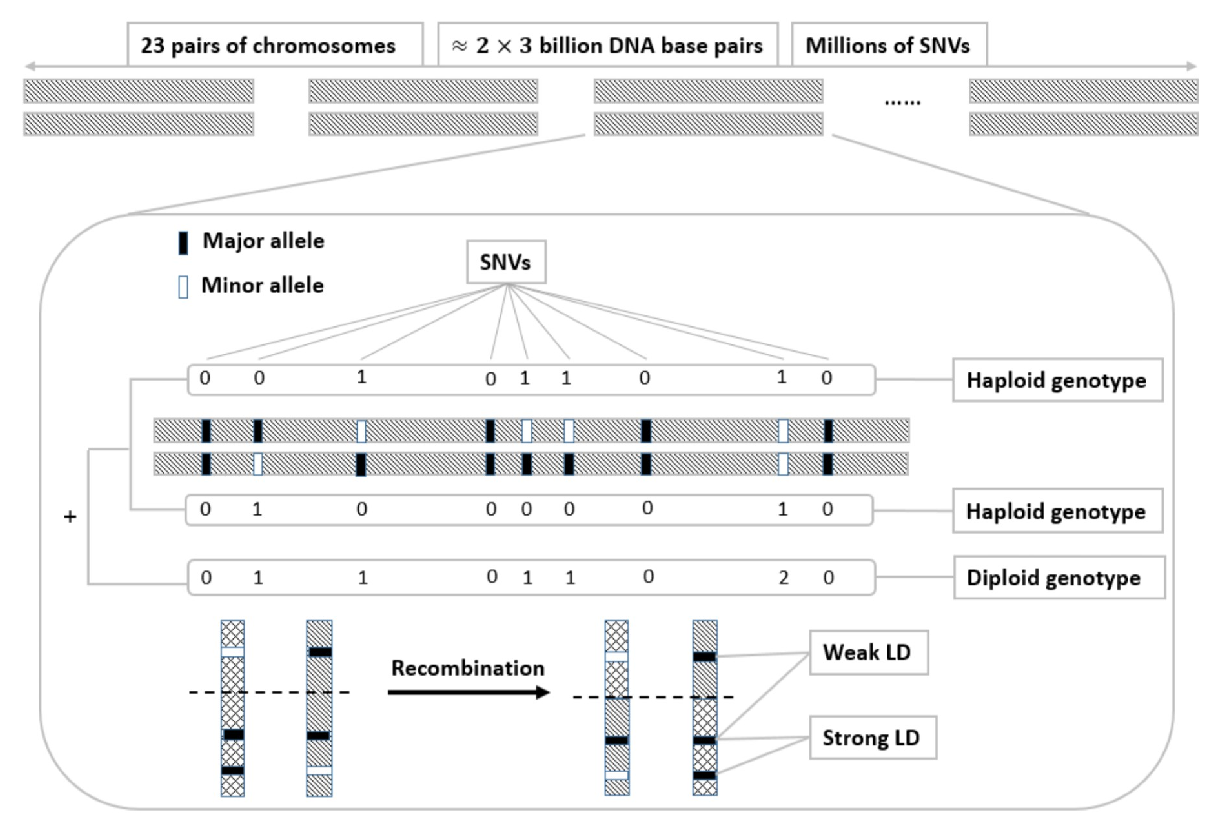
\includegraphics[width = 0.9\linewidth]{./figures/Fig1-human-genomic-overview.eps}
	\caption{人类基因组概览~\cite{samani2015quantifying}
	}
	\label{fig:human-genomic-overview}
\end{figure}

为方便起见,每个SNP位点的三个可能状态(即AA,Aa和aa)分别用0、1和2表示,具体数值取决于每个基因位点上次要等位基因的数量。

连锁不平衡(Linkage disequilibrium,LD)被定义为等位基因在两个或多个位点上的对应关系或非随机关联关系。这种关联关系是遗传机制的结果,即某一个群体有足够的进化时间,基因随机重组的出现将在所有位点产生等位基因的平衡分布。对LD建模的方法有几种,本文中我们主要应用混合建模的LD数据,该建模方法同时考虑了参照基因型数据集和基因重组率的影响。

在遗传过程中,基因重组是一个子过程,在该过程中,一些DNA片段被分离并重新组合,形成新的等位基因组合。基因重组过程产生了所有生物的遗传多样性,基因重组与LD是直接相关的。

\subsection{隐Markov模型}

隐Markov模型(Hidden Markov Model, HMM)~\cite{rabiner1989tutorial,stamp2004revealing}是一种状态不可观测的统计Markov模型,可以通过简单的动态贝叶斯网络表示。具体来说,本章的研究过程中采用了三个假设:(1)~$~t~$~时刻的状态是由某个状态为~$~S_t~$~ 隐藏的过程生成的;(2)该过程具有Markov特性;(3)隐藏的状态变量是离散的。
HMM可用于表征诸如相似性、解码和学习等基本问题。 目前,HMM在语音识别~\cite{rabiner1989tutorial}、手写识别~\cite{hu1996hmm}、基因预测~\cite{durbin1998biological}等领域得到了广泛的应用。

本章考虑的问题在某种程度上类似于参数学习问题。由于在给定观测或发射序列的推断过程中,所有隐藏状态变量的后边缘都可以通过计算得到,因此我们考虑采用正向-反向算法。

\subsection{卷积神经网络}

卷积神经网络(Convolutional Neural Network, CNN)~\cite{long2017fully,scutti2018what}已成为解决图像分类、分割和回归问题的一种流行方法。但是,尚未发现有应用回归CNN(Regressive Convolutional Neural Network,RCNN)体系结构(其中最后一层是回归层的CNN)来预测基因型序列的研究。与传统的分类分割问题不同,CNN的输出是离散值~\cite{scutti2018what},而RCNN的输出是连续的。

本章针对类似于缺失值预测问题,我们设计了用于单倍型序列预测的RCNN架构。首先,使用公开单倍型数据集来训练和测试所提出的RCNN模型。建立RCNN预测模型后,首先将观测到的二倍体基因序列解析为单倍体,进而推断SNP序列上隐藏SNP的基因型,并将其应用于攻击个体的基因型序列隐私信息。


\section{敌手模型与敌手隐私分析能力量化}\label{sec:adver}

\subsection{敌手模型}

本节提出的敌手模型主要针对现实世界中涉及基因组数据共享的场景。在这种情况下,被攻击对象共享其SNP序列用于研究、医学测试或寻找亲属。由于隐私保护的需求,被攻击者希望隐藏某些可能与遗传病或私人特征有关的敏感SNP。因此,被攻击对象共享其原始SNP序列的变体~$\hat{X}=(\hat{x}_1,\hat{x}_2, ... , \hat{x}_n)~$~, 其中~$\hat{x}_i =\{0,1,2\}$~,并隐藏其中某些SNP。假设隐藏的SNP用~$~X_H~$~表示,可观测的SNP用~$~X_O~$~表示,公开的SNP用~$~X=(x_1, x_2, ..., x_n)=X_H \cup X_O~$~,其中~$~x_i =\{-1,0,1,2\}$~,值~$~x_i=-1~$~表示~$~x_i\in X_H~$~是隐藏的SNP。假设已观测被攻击者公开SNP~$~X~$~序列数据的敌手想要重构原始SNP序列~$\hat{X}$~。为此,敌手可以通过推断攻击获取被攻击者的基因组隐私(例如获得其APOE基因状态~\cite{nyholt2009jim})。要进行这样的推断攻击,敌手将收集一些公开可用的基因组信息~\cite{IGSR2019,howie2014impute2},例如被攻击者所属族群的次要等位基因频率(Minor Allele Frequency,MAF)、LD值、遗传重组率和单倍体基因型参照,如图~\ref{fig:adversary-model} 所示。

\begin{figure}[htbp]
	\centering
	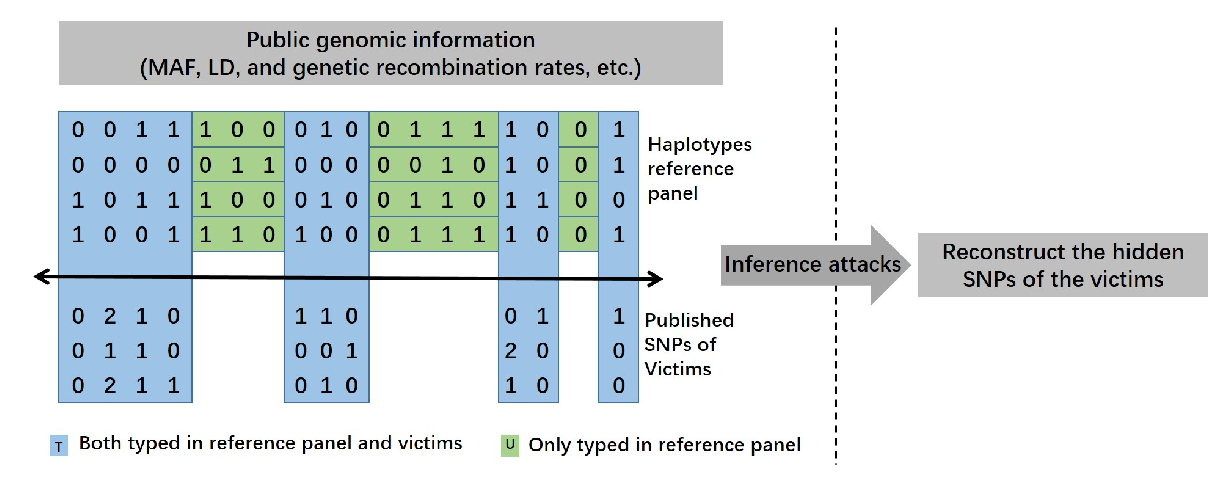
\includegraphics[width = 0.95\linewidth]{./figures/Fig2-adversary-model.eps}
	\caption{基因序列数据属性隐私分析推断敌手模型概览}
	\label{fig:adversary-model}
\end{figure}

假设可访问的公开基因组信息用~${INFOR}_{Pub}$~表示,推断的SNP序列用~$\bar{X}=(\bar{x}_1, \bar{x}_2,...,\bar{x}_n)~$~表示。基于基因型隐私的推断攻击的敌手模型~$~infer~$~可以形式化地表示为
\begin{align}\label{eq:adversary-model}
\bar{X} =& infer(X,{INFOR}_{Pub})  \nonumber \\
= & infer(X_H,H_O,{INFOR}_{Pub}).
\end{align}

更具体地说,基因序列数据属性隐私推断攻击可以看作是给定已发布的SNP和公开基因组信息,计算每个隐藏SNP的条件边缘概率分布的过程,即
\begin{align}\label{eq:adversary-model-prob}
Prob(X=\{0,1,2\})=Prob(X|(X_O,{INFOR}_{Pub})).
\end{align}
对于每个隐藏SNP位点的隐私数值,其预测值是条件概率最高的那个值。

\subsection{敌手隐私分析能力量化标}


为了量化敌手在基因组隐私推断方面的能力,本章使用Ayday等~\cite{ayday2013personal}引入的\textit{基因组隐私度量}方法,从而评估敌手通过推断攻击可以在多大程度上损害被攻击者的基因组隐私。如同Wagner
~\cite{wagner2017evaluating}
所述,有几种不同的基因组隐私度量方法适用于本章的研究。在本章中,假设敌手的目标是隐藏的推断SNP序列的属性隐私值,且仅考虑个体实际拥有的SNP序列。我们应用\textit{正规不正确性}(即敌手的不正确性),\textit{正规熵}(即敌手的不确定性)和\textit{正规互信息}(即被攻击者的隐私损失)来量化推断攻击模型的隐私分析强度。

作为基因组隐私度量,\textit{正规不正确性}可以表示为
\begin{align}\label{eq:metric-correctness}
E=1- \frac{\sum_1^n \mid \bar{x}_j - \hat{x}_j \mid}  {\mid X_H \mid},
\end{align}

其中,~$n$~为被攻击者的SNP数量,~$\bar{x}_j~$~为推断出的SNP在~$~j~$~位点的基因型值,~$\hat{x}_j~$~为SNP在~$~j~$~位点的原始基因型值,~$\mid X_H \mid~$~为属于被攻击者隐藏的SNP数量。

尽管不正确性是衡量隐私权的有力指标,但由于被攻击者SNP的原始值不可用,因此它并不适合许多场景。在这些情况下,我们需要其他指标。在本章中,我们采用\textit{正规熵}来表示敌手的不确定性,该度量可以根据所推导的SNP序列的\textit{正规熵}来评估。特别地,
\begin{align}\label{eq:metric-entropy}
H = \frac{\sum_{j=1}^n \frac{H(X_j)}{log(3)}}{\mid X_H \mid},
\end{align}
其中~$~H(X_j)= -\sum_{\bar{x}_j=\in \{0,1,2\}}{p(\bar{x}_j)log(p(\bar{x}_j))}$~ 为推断出的SNP在~$~j~$~位点的熵,~$~log(3)~$~为~$~j~$~位点SNP的最大熵,~$\mid X_H \mid~$~ 为被攻击者的隐藏SNP数。

该度量标准根据敌手的能力而不是被攻击者的隐私损失来量化敌手在其推断攻击中的置信度。如本文第三章所述互信息可以作为这种度量的基础,为此,我们利用不确定性的递减来表示敌手在推断攻击前后对隐藏SNP序列的不确定性的变化。因此,本章使用正规互信息来量化敌手对被攻击者的平均隐私损失,由于互信息的估计是一个困难性问题,依赖条件概率的分布,故本章利用熵的变化量来估计互信息,即
\begin{align}\label{eq:metric-mutual-information}
I = \frac{\sum_{j=1}^n \frac{H_{MAF}(X_j)}{log(3)}}{\mid X_H \mid}
- H,
\end{align}
其中~$~H_{MAF}(X_j) = -\sum_{x_j=\in \{0,1,2\}}{p_{MAF}(x_j)log(p_{MAF}(x_j))}$~ 表示SNP在~$~j~$~位点的自然熵,~$~p_{MAF}(x_j)~$~为根据MAF数据集SNP发生的概率。公式~\ref{eq:metric-mutual-information} 中定义的度量表示推断攻击引起的熵变化量,从而可以度量推断攻击的强度,它还可以评估被攻击者在推断攻击时的基因组隐私损失。

\section{序列型数据隐私分析推断方法}\label{sec:infer}

在这一节中,对于所使用的敌手模型,我们提出了两种推断攻击策略,一个是基于改进的HMM (iHMM)的隐私推断方法,另一个是基于RCNN模型的隐私推断方法。

\subsection{基于iHMM的隐私分析}

为了提高基因组隐私推断的性能,本节方法不同于文献~\cite{samani2015quantifying}中那样直接推断被攻击者的隐藏的SNP基因型,而是受IMPUTE2 ~\cite{howie2009flexible}基因型插补方法的启发,我们将攻击过程分为三个步骤:(1) 使用Markov链Monte Carlo抽样策略将观测到的被攻击者的SNP序列分阶段转为单倍型;(2) 使用HMM模型分别推断每个被攻击者的隐藏单倍型基因型数值;(3)结合对每个被攻击者推断的单倍型结果,形成推断的基因型序列。


在模型的详细构建中,我们将参照数据集和被攻击者的SNP序列分为~$~T~$~(同时出现在参照数据集和被攻击者中的SNP序列)和~$~U~$~(不出现在被攻击者中,但出现在参照数据集中的SNP序列)。我们假设有~$~n~$~个被攻击者, ~$~H_R^T~$~表示~$~T~$~中SNP序列的参照单倍型集合,~$~H_V^T~$~表示被攻击者在~$~T~$~中观察到的SNP序列的单倍型集合,~$~H_V^U~$~表示与~$~U~$~中SNP序列相对应的被攻击者隐藏的单倍型集合,~$~H_V^T=\{H_{V,1}^T,H_{V,2}^T,..., H_{V,n}^T\}$~表示~$~T~$~中与SNP序列对应的被攻击者单倍型,其中~$~H_{V,i}^T~$~表示第~$~i~$~个被攻击者的单倍型,~$\rho~$~表示群组基因重组映射率。

更具体地说,基于iHMM的推断攻击可以分三个步骤进行,详细说明如下:
\begin{enumerate}
	\item[(1)] 敌手根据观察到的被攻击者的基因型,随机产生~$~H_V^T~$~的单倍型。然后,敌手通过多轮Markov链Monte Carlo迭代更新~$~H_V^T~$~中的单倍型。在每次迭代中,敌手通过从~$~P(H_{V,i}^T|G_{V,i}^T,H_{V,-i}^T,H_R^T,\rho)~$~中抽样来更新第~$~i~$~个被攻击者的阶段性单倍型对~$~H_{V,i}^T~$~。
	\item[(2)] 敌手通过基因重组模型利用HMM模型推断~$~H_V^U~$~中的单倍型。在每次迭代中,敌手根据条件分布~$~P(H_{V,i}^U|H_{V,i}^T, H_R^{T \cup U},\rho)~$~推断第~$~i~$~个被攻击者对应~$~U~$~中的SNP序列的隐藏单倍型对~$~H_{V,i}^U~$~。 
	\item[(3)] 敌手把对每个被攻击者推断出来的单倍型对组合起来,得到被攻击者隐藏的SNP序列的推断基因型。
\end{enumerate}

在步骤(1)中每次迭代的分阶段步骤中,抽样条件为~$~k~$~个最接近的单倍型,其结果由其到第~$~i~$~个被攻击者的汉明距离确定。基于基因重组过程,利用HMM模型来推断计算条件分布,采用Monte Carlo方法重构基因解析空间。因为推断得到的状态空间包含~$~H_R^T~$~中单倍型的所有状态和~$~H_{V,-i}^T~$~中当前猜测的单倍型,所以可以获得更多隐私关联信息。

在步骤(2)中,HMM状态空间包含了所有参照单倍型~$~H_R^{T \cup U}$~,此步骤类似于文献~\cite{samani2015quantifying}中基于基因重组模型的过程,该模型受文献~\cite{marchini2007newa}的启发。然而,我们推断每个被攻击者的单倍型数值,而不是直接推断基因型数值。

步骤(1)至(3)中描述的攻击策略与文献~\cite{samani2015quantifying}中描述的攻击策略不同,后者直接推断隐藏SNP的基因型值。在本章中,敌手结合了Markov链Monte Carlo抽样和HMM推断技术,提高了目标SNP序列的条件分布所获得的隐私分析结果。

\subsection{基于RCNN的隐私分析}

基于RCNN的攻击也分为三个步骤,步骤(1)和(3)与基于iHMM的隐私分析推断攻击是相同的,只有步骤(2)不同。同样地,敌手观测公开基因组信息和被攻击者SNP序列,将基因型分为单倍型,分别推断出隐藏的单倍型对,然后将推断出的单倍型对组合成基因型。在这里,我们将基于RCNN攻击的步骤(2)做说明如下。

我们构造基于RCNN的基因序列属性隐私分析目标模型为
\begin{align}\label{eq:rcnn}
H_{V,i}^U  \leftarrow RCNN(H_{V,i}^T, H_R^{T \cup U}),
\end{align}
其中,给定一个参照单倍型集和一个基于观察到的SNP序列的相位单倍型集,公式~\ref{eq:rcnn}的目标是推断这些隐藏部分的值(即0或1)。由于被攻击者的公开参照单倍型和观察到的SNP序列都属于同一群体(如CEU或CHS~\cite{igsr2015which}),因此这些数据具有相同的特征,可以通过神经网络进行分析。

我们对参照数据~$~H_R^{T \cup U}$~提出了一个RCNN模型,将这些数据分成两组:一组是训练集~$~H_{Rtrain}^{T \cup U}$~,另一组是测试集~$~H_{Rtest}^{T \cup U}$~。然后我们对最小值~$~min(\|H_{Rtest}^{ U} - \hat{H}_{Rtest}^{U}\|)~$~的目标选择最佳训练网络,其中~$\hat{H}_{Rtest}^{U}$~ 表示测试集的预测值。敌手可以使用这个优化的网络来推断被攻击者单倍型的隐藏值,具体过程如图~\ref{fig:rcnn_infer} 所示。

\begin{figure}[htbp]
	\centering
	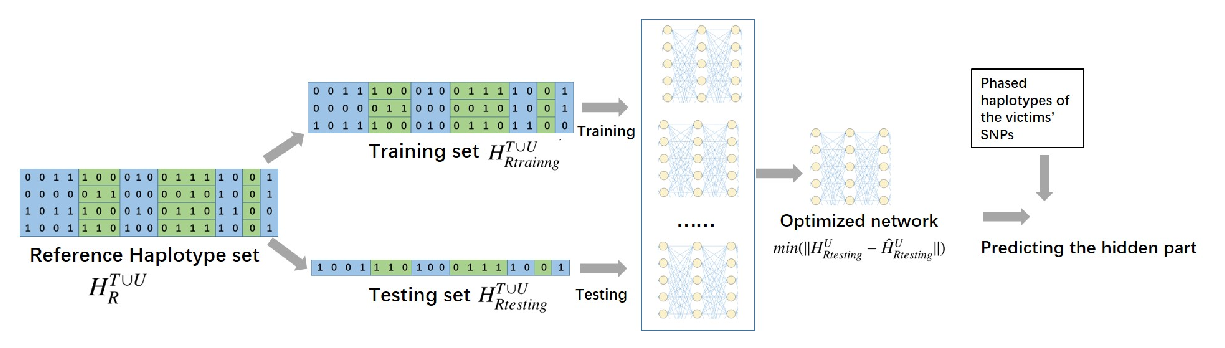
\includegraphics[width=0.95\linewidth]{./figures/Fig3-RCNN-inference-attack.eps}\\
	\caption{基于RCNN的隐私分析模型}
	\label{fig:rcnn_infer}
\end{figure}


\begin{figure}[htbp]
	\centering
	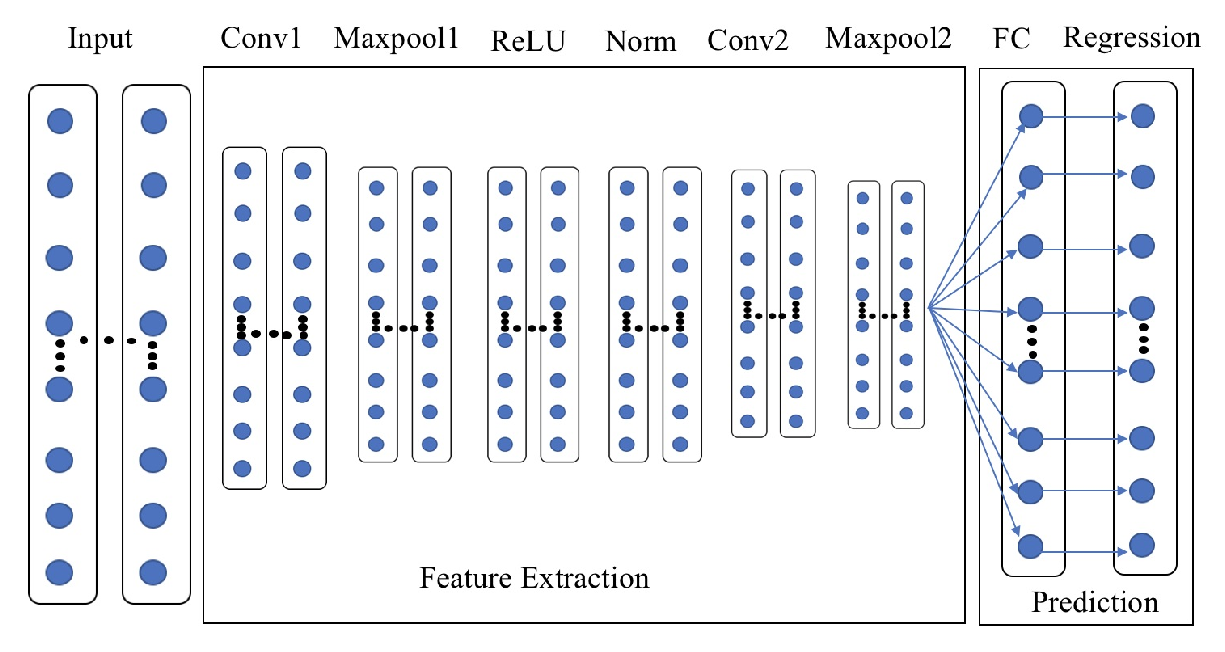
\includegraphics[width=0.7\linewidth]{./figures/Fig4-RCNN-structure.eps}\\
	\caption{基于RCNN的基因隐私分析过程}
	\label{fig:RCNN}
\end{figure}
基于RCNN的基因隐私分析过程如图~\ref{fig:RCNN}所示(其中,Conv为卷积层, NA为正规化层, FC为完全联通层),该过程包含8层网络,输入由观察到的SNP序列的单倍型组成,最后一层回归层生成隐藏SNP序列的单倍体型值。最后一层是代表隐藏SNP序列的单倍型的回归层。在训练阶段,RCNN能够提取基因型的影响因子,检验MES是否收敛。利用RCNN训练得到的分类器,可以对测试数据集中的隐藏SNP序列的单倍型值进行推断。

该网络可实现两项主要任务:特征提取和预测。该网络包括八层,两个卷积层(Conv1和Conv2)、两个最大池层(Maxpool1和Maxpool2)、一个整流线性单元层(ReLU)和一个归一化层(Norm),ReLU层减少了训练所需的时间周期,但是其错误率比传统的双曲正切更高。规范层提高了通用性,降低了错误率。值得注意的是,ReLU层和Norm层并不会改变特征映射的大小。池化层汇总了相邻池化单元的输出。预测步骤完全由连接(FC)层和回归层执行。输入层由~$~8\times 1~$~个影响因子组成(1个月) ,Conv1和Conv2各自的过滤器大小(~$~F~$~)为~$~1\times 1~$~ ,并且过滤器的数量(~$~N~$~)为25,填充大小(~$~P~$~)为0,Maxpool1和Maxpool2的步长(~$~S~$~)为~$~2\times 2~$~。因此,在每个max池层之后,特征图的维数除以2。


为训练RCNN模型,我们最小化损失函数,使用均方误差(MSE)作为损失函数,其定义为
\begin{equation}
\text{Loss}=\frac{1}{N}\sum_{i=1}^{N}|d_{t}^{i}-d_{o}^{i}|^{2},
\end{equation}
其中~$~N~$~是数据集中的条目数,下标~$~i~$~表示数据集中的第~$~i~$~个点位。


如图~\ref{fig:RCNN}所示,一旦在Maxpool2层中提取了额外的特征,我们就可以将其连接到FC层,并将所有的特征压缩成一个维度。在训练过程中,如果在当前迭代次数未达到期望的MSE,则训练将继续进行,直到达到最大的迭代次数或所期望的MSE。如果达到最大迭代次数,则无论MSE值如何,训练过程都会停止。为了验证该方法的可行性和实用性,将测试数据集输入训练好的RCNN模型中,并利用该模型预测隐藏SNP序列的单倍型,从而对总体性能进行评估。


\section{实验与分析}\label{sec:resul}
在本节中,将根据各种指标评估本章提出的序列型数据属性隐私分析推断攻击方法的性能,并基于实验所得到的结果与之前的工作进行比较。

\subsection{数据集选取}
在这些实验选取了来自HapMap项目~\cite{thorisson2005international}第三期的数据集,该数据集在互联网上是公开的。在这个项目中,从世界各地11个不同族群中收集匿名的基因组数据用于基因研究。在不失一般性的前提下,本章采用了2010年5月发布的北欧和西欧祖先(CEU)族群22号染色体的数据集。该数据集包含了个体的单倍型序列,并且还包括了这些群体的MAFs、成对LD值和基因重组率。我们将这些数据视为公开背景数据。此外,HapMap项目数据集中也包含165个个体的基因型序列。本章将使用这些数据作为选择的无关亲属的基因组数据,同时这个数据集也在文献~\cite{samani2015quantifying}中使用过。
\subsection{实验结果对比与分析}

在本节的实验中,随机隐藏被攻击者SNP序列的不同百分比(从5\%到60\%),使用所提出的攻击模型推断隐藏的SNP序列,并根据第~\ref{sec:adver}节中所描述的三个指标量化基因组隐私结果。

首先,随机隐藏10\%的被攻击者的SNP,并使用不同的攻击模型评估敌手的隐私分析推断能力。然后,进行20次实验,取每个量化指标结果的平均值。对基于iHMM和RCNN模型的隐私分析推断攻击强度进行量化计算,敌手的不正确性、敌手的不确定性和被攻击者的隐私损失结果如表~\ref{tab:performance-10per}所示。在此表中,M1-LD,M2和RM分别表示文献~\cite{samani2015quantifying} 中基于一阶Markov链(利用公开二元LD数据),二阶Markov链和基因重组模型的推断攻击,而iHMM和RCNN分别表示基于iHMM和RCNN模型的推断攻击。在错误率列中比较了不同推断攻击的不正确性,本章提出的两种方法结果都显示出在不正确性指标上明显降低,与RM方法相比,iHMM的性能更好,而RCNN的性能稍差。因为文献~\cite{samani2015quantifying} 中的作者在其论文中没有考虑不确定性和隐私损失的度量,所以本节根据计算这两个度量的需要,对其实验进行了改进。结果表明,这两种度量方法同样适用于基因组隐私的度量,在表~\ref{tab:performance-10per}的正规熵列和正规隐私损失列中分别显示了不确定性和隐私损失方面的性能结果。结果表明,利用基于iHMM的推断攻击,敌手可以获得较低的不确定性,并获得更多被攻击者的隐私信息。

为了进一步支撑比较结果,并与文献~\cite{samani2015quantifying}中提出的实验保持一致,本节进行了另一个含有40\%隐藏SNP序列的实验。性能结果如表~\ref{tab:performance-40per}所示,结果表明与表~\ref{tab:performance-10per}中的结论一致,本章所提出的隐私分析方法能够在各种指标对比下获得更好的优势。

\begin{table}[htbp]
	\caption{当10\%SNP序列被隐藏时,不同基因隐私分析推断效果对比}
	\label{tab:performance-10per}
	\begin{tabular}{lccc}
		\hline
		& Error rate & Normalized entropy & Normalized privacy loss\\
		\hline
		M1-LD (Samani et al.) & 0.3356  & 0.4872 & 0.1864 \\
		M2 (Samani et al.)    & 0.2400  & 0.3419 & 0.3316\\
		RM (Samani et al.)    &  0.0578 & 0.069 & 0.6046 \\
		iHMM (Ours)          & 0.0085  &0.0295 & 0.6520 \\
		RCNN (Ours)          & 0.0753  &0.0973 & 0.5143\\
		\hline
	\end{tabular}
\end{table}


\begin{table}[htbp]
	\caption{当40\%SNP序列被隐藏时,不同基因隐私分析推断效果对比}
	\label{tab:performance-40per}
	\begin{tabular}{lccc}
		\hline
		& Error rate & Normalized entropy & Normalized privacy loss \\
		\hline
		M1-LD (Samani et al.) & 0.3623 & 0.4867 & 0.1873 \\
		M2 (Samani et al.)    & 0.2873 & 0.3489 & 0.3251 \\
		RM (Samani et al.)    & 0.0923 & 0.0902 & 0.5838 \\
		iHMM (Ours)          & 0.0136 & 0.0430 & 0.6342 \\
		RCNN (Ours)          & 0.1028 & 0.1345 & 0.5347\\
		\hline
	\end{tabular}
\end{table}

\begin{figure}[htbp]
	\centering
	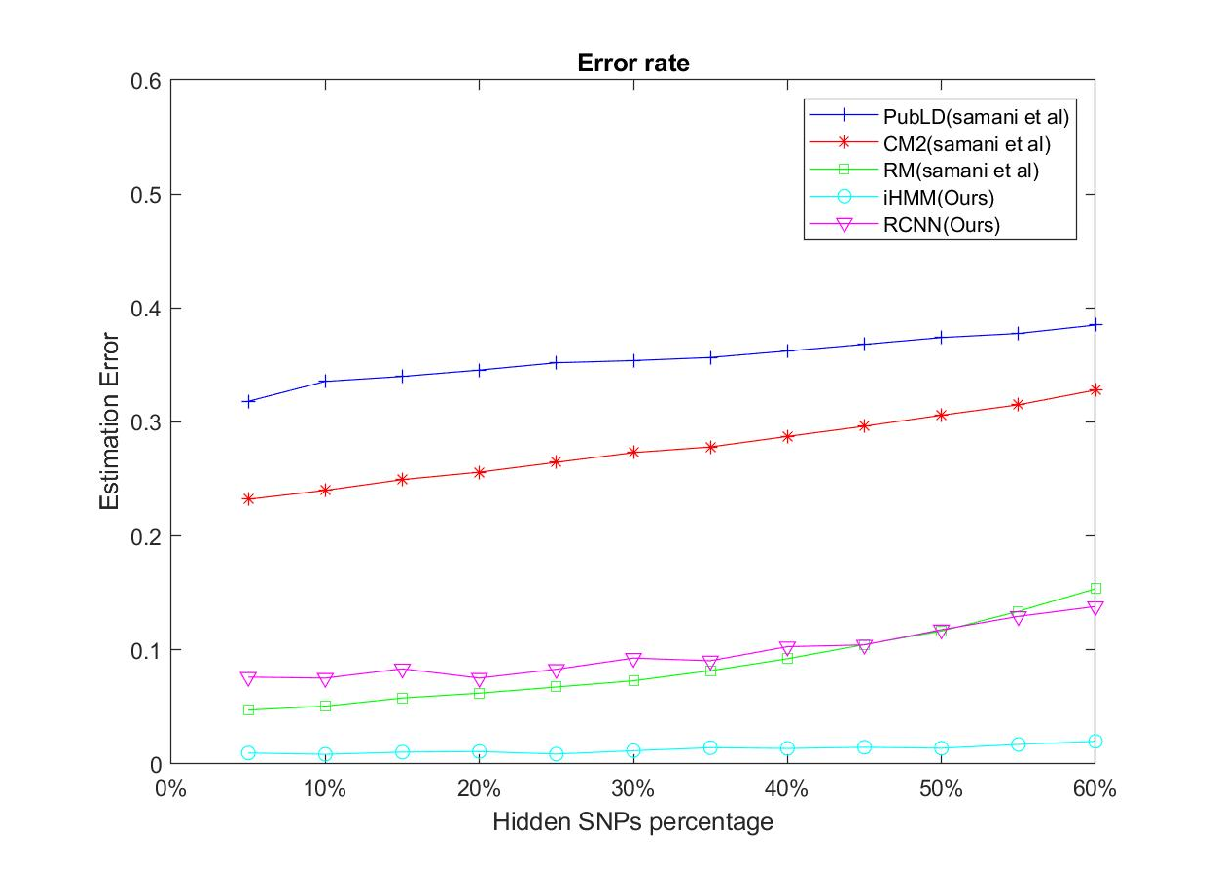
\includegraphics[width =0.8\linewidth]{./figures/Fig5-genomic-privacy-quantifying-incorrectness.eps}
	\caption{不同基因隐私分析模型的基因组隐私变化对比(攻击者错误率)}
	\label{fig:error}
\end{figure}
\begin{figure}[htbp]
	\centering
	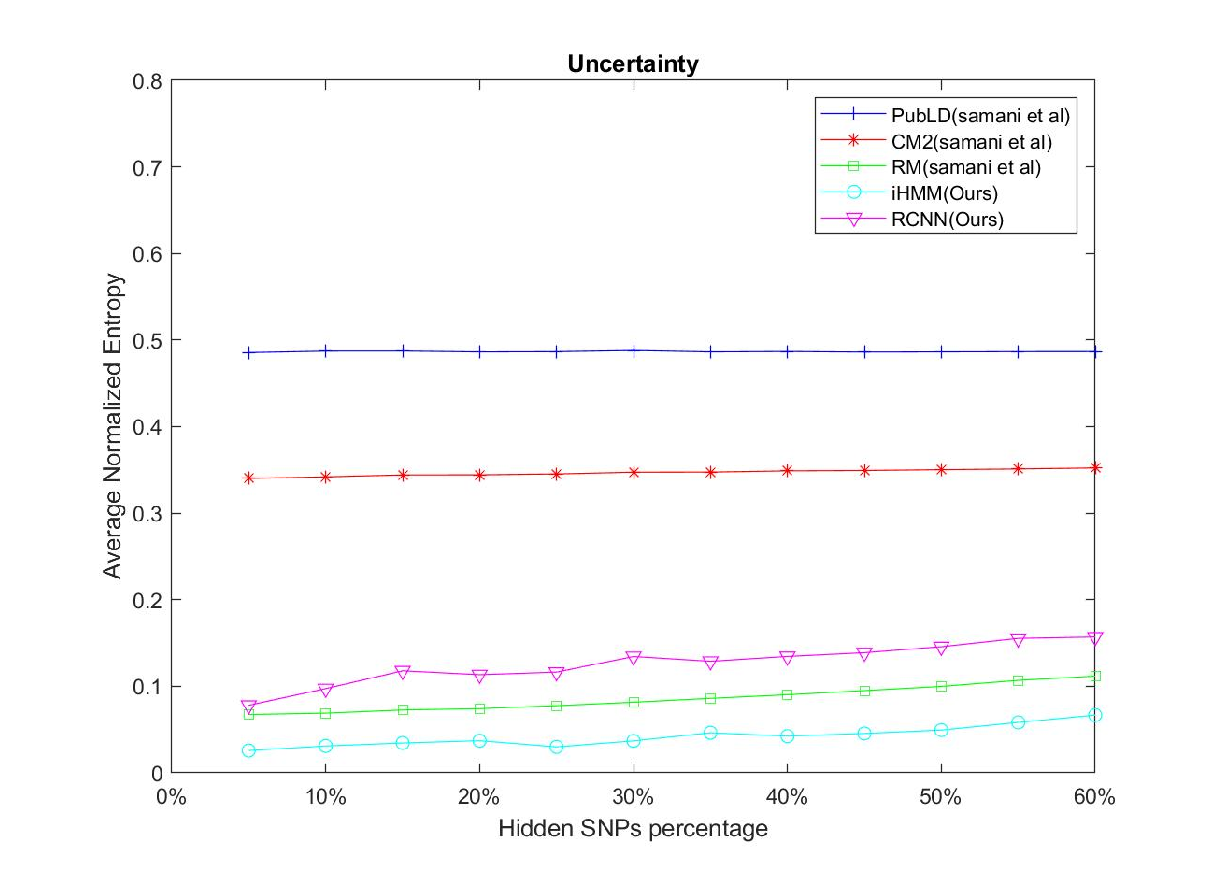
\includegraphics[width =0.8\linewidth]{./figures/Fig6-genomic-privacy-quantifying-uncertainty.eps}
	\caption{不同基因隐私分析模型的基因组隐私变化对比(攻击者不确定性)}
	\label{fig:uncertainty}
\end{figure}
\begin{figure}[htbp]
	\centering
	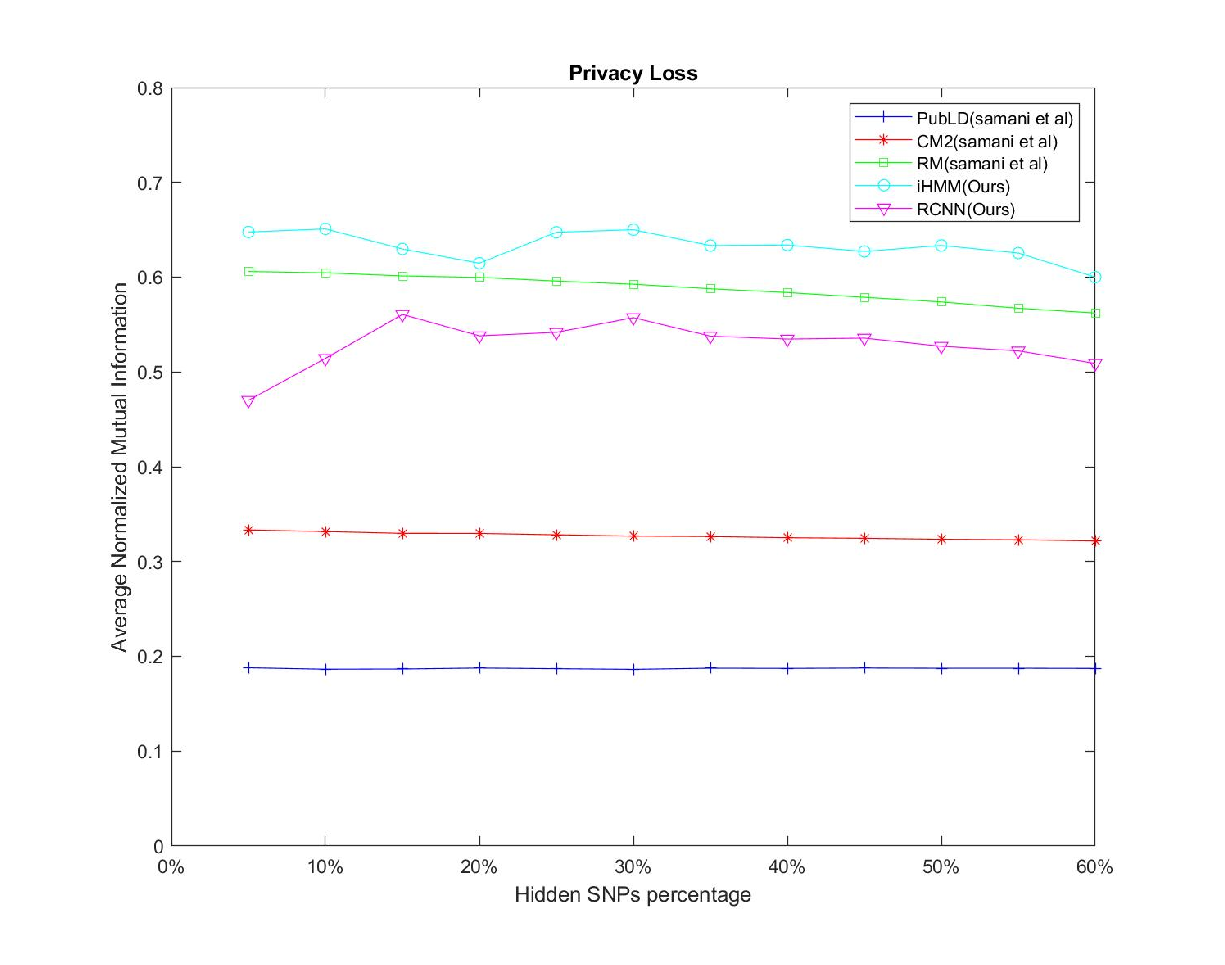
\includegraphics[width =0.8\linewidth]{./figures/Fig7-genomic-privacy-quantifying-privacyloss.eps}
	\caption{不同基因隐私分析模型的基因组隐私变化对比(被攻击者隐私损失角度)}
	\label{fig:privacyloss}
\end{figure}

接下来,为了观察隐藏SNP序列数量对不同推断攻击的影响,本节又进行了一组实验,实验中使用了不同比例(5\% - 60\%)的隐藏SNP序列对LD、2阶Markov链、重组模型、iHMM和RCNN攻击。敌手的不正确性、敌手的不确定性和敌手的基因组隐私损失结果分别如图~\ref{fig:error}、图~\ref{fig:uncertainty}和图~\ref{fig:privacyloss}所示。

在图~\ref{fig:error}中,根据敌手的不正确性展示了基于不同模型的推断攻击的结果。当被攻击者少量的SNP序列被隐藏时,可以发现这些攻击的推断能力会增加(即,被攻击者的SNP序列暴露给敌手的越多,不正确性越低)。与之前的工作相比所提出的两种攻击模型在不正确性方面均显示出更好的推断能力。当隐藏更多SNP序列(大于50\%)时,基于RCNN的攻击性能优于基于重组模型的攻击;当隐藏更少SNP序列时(小于45\%)时,基于重组模型的攻击性能略差。

在图~\ref{fig:uncertainty}中,根据敌手的不确定性显示了基于不同模型的推断攻击的结果。可以看出,当被敌手隐藏的SNP序列越少时,这些攻击的推断能力越强(即,被攻击者的SNP序列暴露给敌手的越多,不确定性越低),结果与图~\ref{fig:error}的结果一致。对比表明,基于iHMM的攻击总是比其他攻击效果更好,而基于RCNN的攻击效果并非始终都是好的。

同样的,在图~\ref{fig:privacyloss}中的结果可以看到被攻击者隐私损失的结果。同样,当被攻击者隐藏的SNP越少,这些攻击的推断能力就越强(即被攻击者的SNP序列暴露给敌手的越多,隐私损失越大)。

\section{小结}\label{sec:concl}

本章提出了两种针对序列型基因数据的隐私分析攻击方法,通过改进的隐Markov模型或回归卷积神经网络模型,利用网络公开基因组信息和个体的部分公开共享SNP序列数据推断个体的隐私基因型信息。研究表明,敌手能够准确、低不确定性和高隐私损失地推断出个体的私有隐藏SNP隐私信息。实验表明,所提出的攻击扩展并显著改进了现有的工作。通过基于公开的基因组数据对个体基因组隐私进行量化,本章的工作可以帮助人们更好地理解当前基因组隐私面临的风险,促进隐私领域更加小心地应用基因组数据,促进研究人员设计更好的隐私保护模型()如后文研究的基于风险访问控制模型)以适应性地保护基因序列数据隐私。

